\documentclass[a4paper, 12pt]{article}
\usepackage{listings} 
\usepackage{xcolor}
\usepackage{mdframed}
\usepackage{graphicx}
\usepackage{pgfplots}
\usepackage{float}
\usepackage{mathtools}
\usepackage[margin=1.00in]{geometry}
\DeclarePairedDelimiter\ceil{\lceil}{\rceil}
\DeclarePairedDelimiter\floor{\lfloor}{\rfloor}
\definecolor{code-gray}{gray}{0.93}

% Beginning of Document
\begin{document}

% Title
\title{ECE 443 - Project \#4}
\author{Collin Heist}
\date{\today}
\maketitle

% Table of Content and Listings
\pagenumbering{roman}
\tableofcontents
\lstlistoflistings
\newpage
\pagenumbering{arabic}

% Beginning of Report
\section{Tracealyzer Utilization}

\subsection{Heartbeat Tracealyzer}
To begin with, the project guidelines give pretty clear instructions on what components to add to the project. We're told (quite explicitly) to add a change-notice interrupt generation task, a change notice handler task, an LCD write task, and a LEDA toggling task. I chose to implement my IR sensor reading as a separate \emph{library} file. 

Because of the clear segmentation of the project, I decided to create three Tracealyzer channels. I have one for logging change notice events, another for logging LCD related events, and a final channel for logging the heartbeat task events.

The (presumably) easiest to implement was the heartbeat task. This is a zero-priority task that utilizes a non-API call way of delaying itself (so that it's always \emph{ready}). This is my code for that:

	\begin{mdframed}[backgroundcolor=code-gray, roundcorner=10pt,
								innerleftmargin=5, innertopmargin=5, innerbottommargin=5]	
	\begin{lstlisting}[language=C, caption=Heartbeat Task, tabsize=2, label={lst:task-leda-toggle}]
	static void task_leda_toggle(void* task_params) {
		unsigned int t_wait, t_start;
	
		for (;;) {
			t_start = ReadCoreTimer();
			t_wait = CORE_MS_TICK_RATE * LEDA_TOGGLE_MS;
			while (ReadCoreTimer() - t_start < t_wait);
			LATBINV = LEDA;
			if (configUSE_TRACE_FACILITY)
				vTracePrint(trace_leda_toggle, "Toggled LEDA");
		}
	}
	\end{lstlisting}
	\end{mdframed}
	
I utilized Tracealyzer here to verify that the toggling task was executing properly. However, this was a bit superfluous as Tracealyzer automatically logs any task-switches, resulting in a log of the toggle anyway. However, after this allowed me to verify that my heartbask task was executing properly (on its own). 

\subsection{Change Notice Tracealyzer}
Next, I added in the change notice functionality. We were told to add a change notice ISR that was triggered by a task that sets the change notice flag every 5 milliseconds. I utilized my Tracealyzer channel, \textbf{trace\_cn}, to note the important events in this sequence of events. For starters, inside the handler is the code shown in \textbf{Listing~\ref{lst:isr-change-notice-handler}}.

	\begin{mdframed}[backgroundcolor=code-gray, roundcorner=10pt,
								innerleftmargin=5, innertopmargin=5, innerbottommargin=5]	
	\begin{lstlisting}[language=C, caption=Change Notice ISR, tabsize=2, label={lst:isr-change-notice-handler}]
	void isr_change_notice_handler() {
		portBASE_TYPE move_to_higher_priority = pdFALSE;

		if (configUSE_TRACE_FACILITY)
			vTracePrint(trace_cn, "Giving semaphore from CN ISR");
		xSemaphoreGiveFromISR(cn_semaphore, &move_to_higher_priority);

		mCNClearIntFlag();
		mCNOpen(CN_OFF, (CN8_ENABLE), 0);

		portEND_SWITCHING_ISR(move_to_higher_priority);
	}
	\end{lstlisting}
	\end{mdframed}
	
As you can see, I used Tracealyzer here to notify when the semaphore is being given, which (ideally) should prompt a transition into the change notice handler task (shown in \textbf{Listing~\ref{lst;task-change-notice-handler}}).

	\begin{mdframed}[backgroundcolor=code-gray, roundcorner=10pt,
								innerleftmargin=5, innertopmargin=5, innerbottommargin=5]	
	\begin{lstlisting}[language=C, caption=Change Notice Handler Task, tabsize=2, label={lst:task-change-notice-handler}]
	static void task_change_notice_handler(void* task_params) {
		float temp = 0.0;
		char lcd_message[LCD_WIDTH+1] = {0};
		portBASE_TYPE queue_status;
	
		xSemaphoreTake(cn_semaphore, 0);
		for (;;) {
			xSemaphoreTake(cn_semaphore, portMAX_DELAY);
			if (configUSE_TRACE_FACILITY)
				vTracePrint(trace_cn,
				"Received semaphore, reading from IR sensor");
		
			temp = read_ir_temp();
			if (temp == ERROR_TEMP) {
				if (configUSE_TRACE_FACILITY)
					vTracePrint(trace_cn, "Error in temperature reading");
			}
			else {
				if (configUSE_TRACE_FACILITY)
					vTracePrint(trace_cn,
						"Temperature read successfully - adding to Queue");
				sprintf(lcd_message, "Temp: %3.1f", temp);
			
				queue_status = xQueueSendToBack(lcd_string_queue,
					&lcd_message, portMAX_DELAY);
				if (configUSE_TRACE_FACILITY && queue_status == errQUEUE_FULL)
					vTracePrint(trace_cn,
						"Unable to add to Queue, Queue is full");
			}
		}
	}
	\end{lstlisting}
	\end{mdframed}
	
Once again, I used the change notice Tracealyzer channel to mark significant events as they occur. In this instance that is receiving the semaphore, reading from the IR sensor, whether there was an error in the temperature reading or not, and if adding to the queue went properly. This allowed me to easily see the sequence of events occuring when a read was initiated by the change notice interrupt being set. This sequence of events is particularly evident in my Tracealyzer output, where the various channels can be seen handing off to each other. See this sequence of events inside \textbf{Figure~\ref{fig:operation-log}}.

\subsection{LCD Tracealyzer}
Finally, the LCD operations had their own Tracealyzer channel. This was used entirely by the task being used to write to the LCD, and only notified the user when a pointer was received from the Queue, and when the message was written to the LCD. Again, this is shown below.

	\begin{mdframed}[backgroundcolor=code-gray, roundcorner=10pt,
								innerleftmargin=5, innertopmargin=5, innerbottommargin=5]	
	\begin{lstlisting}[language=C, caption=LCD Task, tabsize=2, label={lst:task-display-lcd}]
	static void task_display_lcd(void* task_params) {
		char lcd_message[LCD_WIDTH+1] = {0};
		unsigned int i = 0;
		for (;;) {
			xQueueReceive(lcd_string_queue, &lcd_message, portMAX_DELAY);
			if (configUSE_TRACE_FACILITY)
				vTracePrint(trace_lcd,
					"Received pointer from Queue - writing to LCD");
		
			set_cursor_LCD(FIRST_LINE_START);
			put_string_LCD(lcd_message);
			if (configUSE_TRACE_FACILITY)
				vTracePrint(trace_lcd,
					"Message written to LCD, waiting for value in Queue");
		
			for (i = 0; i < LCD_WIDTH + 1; i++)
				lcd_message[i] = '\0';
		}
	}
	\end{lstlisting}
	\end{mdframed}
	
\section{Testing \& Verification}
Adding these Tracealyzer channels made verifying my program's behavior very easy. In particular, it showed me a problem with the heartbeat task. The Tracealyzer view showed that the LEDA toggling task was only being executed every 5 milliseconds -- when the project requirements asked for 3 milliseconds. Luckily, the Tracealyzer event log also revealed why this was happening, as well. It was evident that the low-priority heartbeat task was being executed enough, but was being interrupted by the higher-priority change-notice generator, and LCD writing tasks. These tasks take a significant amount of time (on the order of 2.5 milliseconds, according to Tracealyzer), and therefore prolonged the heartbeat task from toggling by that length of time.

Given the design restrictions, there is no fix to this. The clock frequency of the IR sensor is maxed at 100 kHz, and still the writing simply takes too long. But, this did showcase the utility of Tracealyzer, as I would not have easily been able to diagnose this problem without it.

\section{Figures}
In the below figure, it is quite evident that the desired sequence of events are occurring as expected. To begin, the ISR is entered for a \emph{very} small amount of time, prompting the transfer to the change notice handler, and then the change notice task.

Inside the ISR task (it can be seen on the left side of the \textbf{Figure}, the red Actor), the semaphore is given and then a \textbf{vTaskDelayUntil()} is called. After this the change notice handler, the yellow Actor, takes the semaphore, reads the temperature and adds the string pointer to the queue. Finally, the display task (the green task), receives from that queue and the message is written to the LCD.

I've included the vertical trace view of the LCD writing operation to showcase how long it takes to perform the write. Just over 2 milliseconds are spent \emph{just} writing to the LCD, and given the additional overhead for generating the change notice, reading from the IR sensor, and adding to the queue, it's quite clear that the desired 3 millisecond heartbeat toggle is unachievable in this lab (without adding pauses during the operation of the LCD writing task).

\begin{figure}[H]
\centering
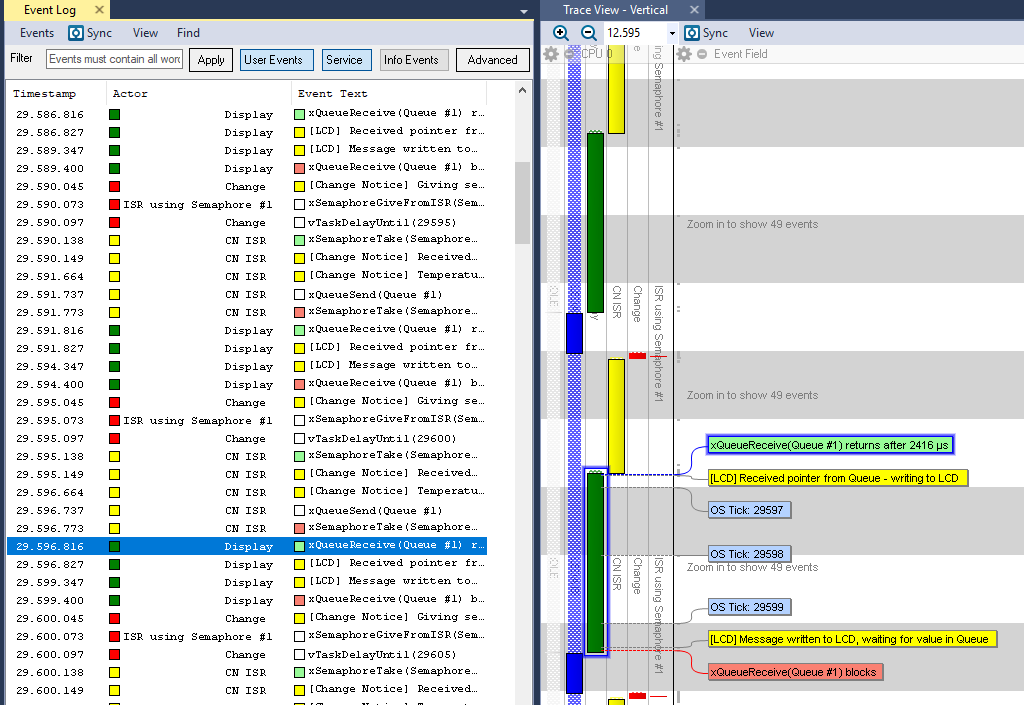
\includegraphics[width=\textwidth]{Operation.PNG}
\caption{TraceAlyzer log of the program's operation}
\label{fig:operation-log}
\end{figure}

\end{document}